\chapter{The Histogram of Gradient Orientations of Signal Plots}
\label{chapter:three}
In this section the generalities of the method will be described.

\section{Introduction}

Image transformation and variants to transform a signal into an image.

sinuplot, spectrogram, scalogram


The research that encompass how to extract information 

The work of Edelman, Intrator and Poggio 1997 how the visual cortex sees features was the inspiration to the use of the histogram of gradient orientations to 

\section{Feature Extraction: Histogram of Gradient Orientations}
\label{SIFT}


On the generated image $I$, a keypoint $\mathbf{kp}$ is placed on a pixel $(x_{kp}, y_{kp})$ over the image plot and a window around the keypoint is considered. A local image patch of size $S_p \times S_p$ pixels is constructed by dividing the window in $16$ blocks of size $3s$ each one,  where $s$ is the scale of the local patch and it is an input parameter of the algorithm. It is arranged in a $4 \times 4$ grid and the pixel $ \mathbf{kp}$ is the patch center, thus $S_p = 12s $ pixels. 

A local representation of the signal shape within the patch can be described by obtaining the gradient orientations on each of the $16$ blocks and creating a histogram of gradients.  This technique is based on Lowe's SIFT~\cite{Lowe2004} method, and it is biomimetically inspired in how the visual cortex detects shapes by analyzing orientations~\cite{cogprints561}.   In order to calculate the histogram, the interval $[0-360]$ of possible angles is divided in $8$ bins, each one at $45$ degrees.

 Hence, for each spacial bin $ i,j = \{0,1,2,3\} $, corresponding to the indexes of each block $B_{i,j}$,  the orientations are accumulated in a  $3$-dimensional histogram $h$ through the following equation: 
 

\begin{equation}
 h(\theta,i,j) = 3 s \sum_{\mathbf{p}} w_\mathrm{ang}(\angle J(\mathbf{p}) - \theta)\, w_{ij}\left(\frac{\mathbf{p} - \mathbf{kp}}{3 s}\right)\, |J(\mathbf{p})|
\label{eq:histogram}
\end{equation}

\noindent  where $\mathbf{p}$ is a pixel from within the patch,  $\theta$ is the angle bin with $ \theta \in \{0, 45, 90, 135, 180, 225, 270, 315\} $,  $ |J(\mathbf{p})| $ is the norm of the gradient vector in the pixel $\mathbf{p}$ and it is computed using finite differences and $\angle J(\mathbf{p}) $ is the angle of the gradient vector.  The scalar $ w_\mathrm{ang}(\cdot) $  and vector $ w_{ij}(\cdot) $ functions are linear interpolations used by~\cite{Lowe2004} and \cite{Vedaldi2010} to provide a weighting contribution to eight adjacent bins.  They are calculated as  

\begin{equation}
 w_{ij}(\mathbf{v}) = w( v_x - x_i ) w( v_y - y_i ) 
\label{eq:ij}
\end{equation}

\begin{equation}
 w_\mathrm{ang}(\alpha) = \sum_{k} w( \frac{8\alpha}{2\pi} + 8r)
\label{eq:wang}
\end{equation}

\noindent where $x_i$ and $y_i$ are the spatial bin centers located in $ x_i,y_i = \{-\frac{3}{2},-\frac{1}{2},\frac{1}{2},\frac{3}{2}\} $, $\mathbf{v} = ( v_x, v_y ) $ is a dummy vector variable and $\alpha$ a dummy scalar variable.  On the other hand, $r$ is an integer that can vary freely which allows the argument $\alpha$ to be unconstrained in terms of its values in radians. The interpolating function $w(\cdot)$ is defined as:

\begin{equation}
 w(z) = \max(0,|z|-1)
\label{eq:weighting}
\end{equation}

These binning functions conform a trilinear interpolation that has a combined effect of sharing the contribution of each oriented gradient between their eight adjacent bins in a tridimensional cube in the histogram space, and zero everywhere else.

Lastly, the fixed value of $ 3 $ is a magnification factor which corresponds to the number of pixels per each block when $s = 1$.  As the patch has  $16$ blocks and  $8$ bin angles are considered, a feature called \textit{descriptor} of $128$ dimension is obtained. 
%It can be observed that the histogram is computed by multiplying by $ |J(\mathbf{p})| $, so the method considers both, the magnitude and the orientation of the gradient vector. 

Fig.~\ref{fig:sampledescriptor} shows an example of a patch and a scheme of the histogram computation. In (A) a plot of the signal and the patch centered around the keypoint is shown. In (B) the possible orientations on each patch are illustrated.  Only the upper-left four blocks are visible.  The first eight orientations of the first block, are labeled from $1$ to $8$ clockwise. The orientations of the second block $ B_{1,2} $ are labeled from $9$ to $16$.  This labeling continues left-to-right, up-down until the eight orientations for all the sixteen blocks are assigned. They form the corresponding $\mathbf{kp}$-descriptor of $128$ coordinates. Finally, in (C) an enlarged image plot is shown where the oriented gradient vector for each pixel can be seen.

\begin{figure}[h!]
\centering
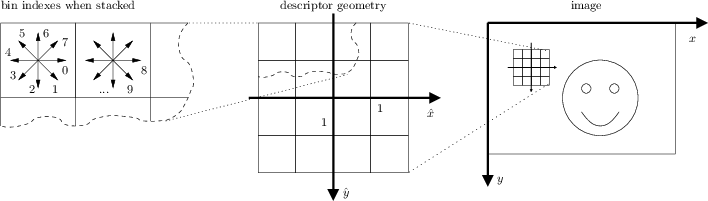
\includegraphics[scale=1.2]{images/sift-conv-vlfeat.png}
\caption[SIFT Patches]{fdsfdfsfs }
\label{fig:siftpatch}
\end{figure}

\begin{figure}[h!]
\centering
\subfigure[10-Fold Cross-validated accuracies values for subject number 12, using Runs 1 and 2 of the Alphanet Dataset.]
{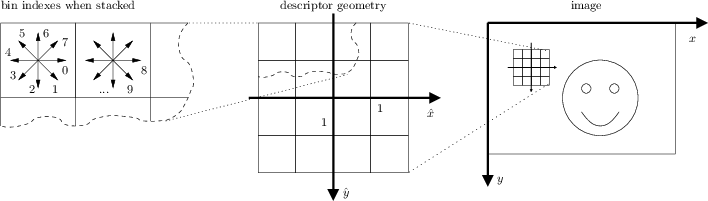
\includegraphics[width=7.5cm, height=5cm]{images/sift-conv-vlfeat.png}}
\subfigure[10-Fold Cross-validated accuracies for O1, Oz, O2 and Iz channels for 25 subjects of the Alphanet Dataset.]
{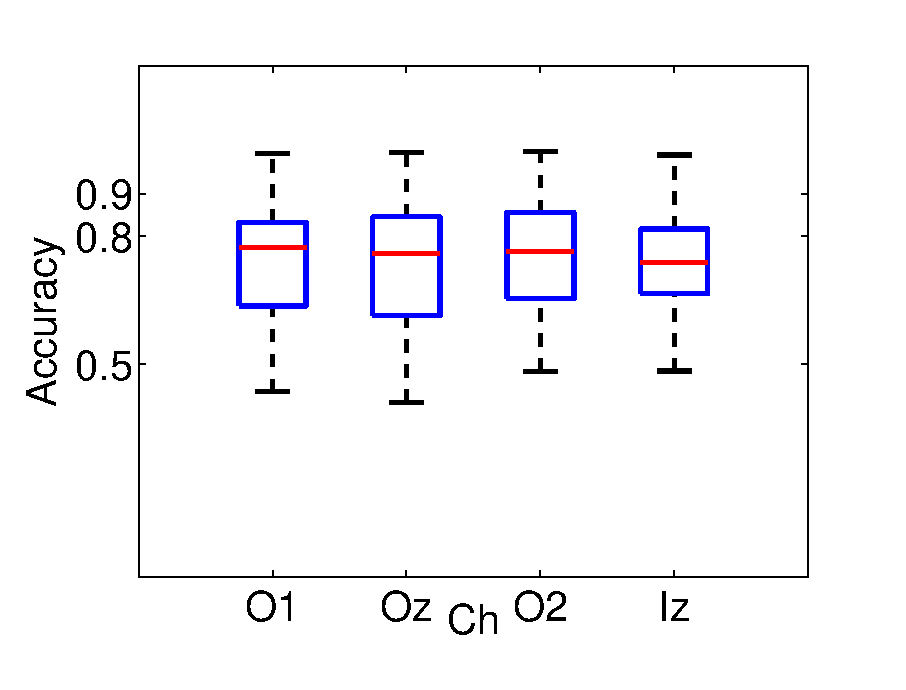
\includegraphics[width=7.5cm, height=5cm]{images/DatasetPhysionetBoxPlots}}
\caption[Alpha Waves Classification]{Classification Accuracy for discriminating windows of 1s (160 samples) of EEG for Alpha Waves differences between subjects with eyes opened and closed. The descriptor size is 12x12 pixels. (Left) 10-Fold cross validated accuracies for one subject.  (Right) Average accuracy levels for 25 subjects for the occipital channels. Medians were above $75\%$.}
\label{fig:alpharesults}
\end{figure}

\section{Keypoint Location}

\section{Oscillatory Processes}

\section{Transient Events}

\section{Mapping Functions}


$\gls{N}$, 
$\gls{lambda}$
$\gls{Fs}$
$\gls{Deltas}$
$\gls{DeltamuV}$
$\gls{gamma}$
$\gls{gammat}$
$\gls{Hy}$
$\gls{Wx}$
$\gls{St}$
$\gls{Sv}$
$\gls{Sy}$
$\gls{Sx}$
$\gls{w}$
$\gls{kp}$
$\gls{P}$

The initial parameters are $N$,$F_s$ and $\lambda$.  The unit length of the patch is $\Delta_s = \sqrt{2} \; 15$.  The peak-to-peak amplitude of the waveform to study is $ \Delta \mu V $.

Amplitude scale factor

\begin{equation}
\gamma \equiv \frac{H_y}{\Delta \mu V}  
\label{eq:gammadefinition}
\end{equation}

Time scale factor

\begin{equation}
\gamma_t \equiv \frac{W_x}{F_s \; w}  
\label{eq:gammatdefinition}
\end{equation}

%\begin{equation}
%s_x = \frac{ \gamma \;  \lambda \  F_s}{12}
%\label{eq:mapping2}
%\end{equation}
%
%\begin{equation}
%s_y= \frac{\gamma \; \Delta \mu V}{12} 
%\label{eq:mapping1}
%\end{equation}

Restriction on the waveform time scale

\begin{equation}
\frac{W_x-1}{\sqrt{2} \; 15}  \geq S_t 
\label{eq:restriction1}
\end{equation}

Restriction on the waveform amplitude scale

\begin{equation}
\frac{H_y-1}{\sqrt{2} \; 15}  \geq S_v 
\label{eq:restriction2}
\end{equation}

Waveform time scale

\begin{equation}
S_t = \frac{ \lambda \;  \  F_s \ \gamma_t }{\Delta_s}
\label{eq:mapping2}
\end{equation}

Waveform amplitude scale

\begin{equation}
S_v= \frac{\Delta \mu V \ \gamma}{\Delta_s} 
\label{eq:mapping1}
\end{equation}

Time to sample point conversion

\begin{equation}
n = \left\lfloor F_s \ \Delta_t \right\rfloor \ \gamma_t
\label{eq:mapping1}
\end{equation}

Horizontal Patch scale

\begin{equation}
\mathbf{S}_x = \Delta_s \; S_t + 1
\label{eq:mapping2}
\end{equation}

Vertical Patch scale

\begin{equation}
\mathbf{S}_y = \Delta_s \; S_v + 1
\label{eq:mapping1}
\end{equation}

Span of a Patch

\begin{equation}
\Delta_t = \frac{S_t \ \Delta_s}{F_s \ \gamma_t} 
\label{eq:mapping1}
\end{equation}


\section{Implementation}

\subsection{Matlab}

\section{Classification}

NBNN

\begin{figure}[h!]
\centering
\subfigure[Classification Method, first step. ]
{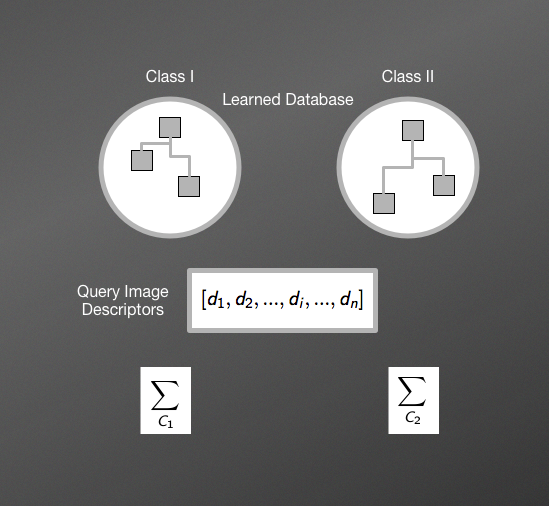
\includegraphics[height=4cm,width=4cm]{images/NBNNMethod1.png}}
\subfigure[Classification Method, first step. ]
{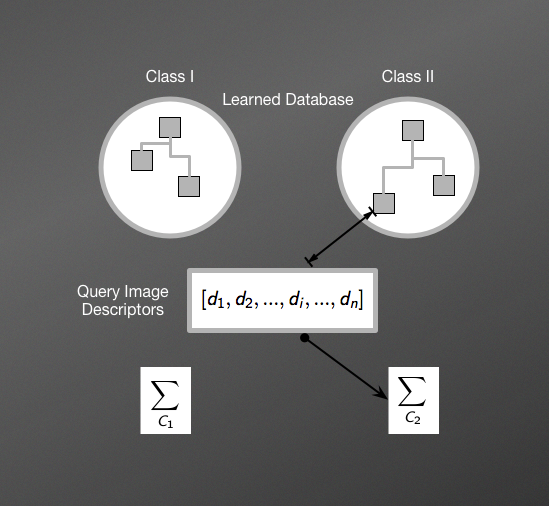
\includegraphics[height=4cm,width=4cm]{images/NBNNMethod2.png}}
\subfigure[Classification Method, first step. ]
{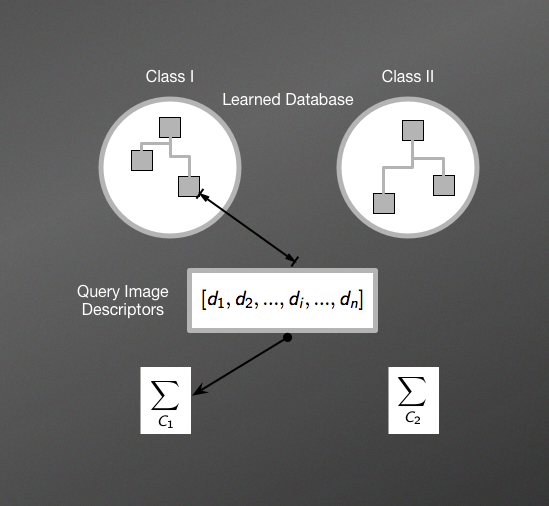
\includegraphics[height=4cm,width=4cm]{images/NBNNMethod3.png}}
\subfigure[Classification Method, first step. ]
{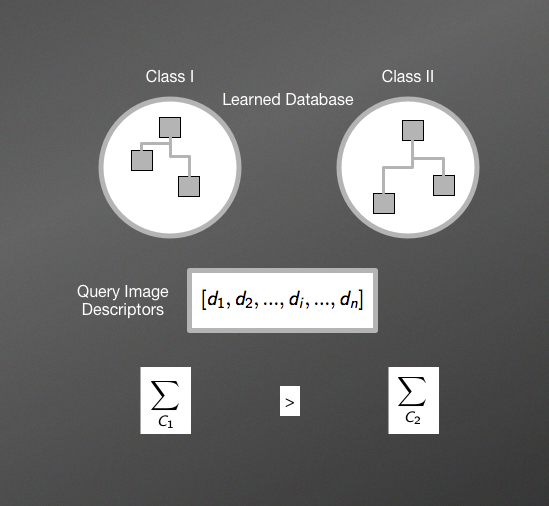
\includegraphics[height=4cm,width=4cm]{images/NBNNMethod4.png}}
\subfigure[Classification Method, first step. ]
{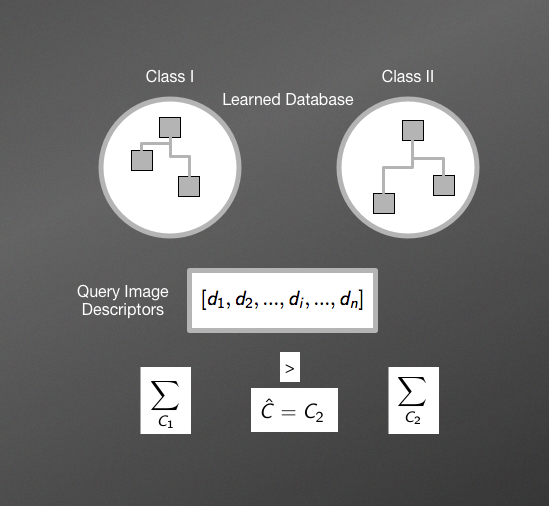
\includegraphics[height=4cm,width=4cm]{images/NBNNMethod5.png}}
\caption[NBNN Classification]{Classification Method.}
\label{fig:nbnnclassification}
\end{figure}



